\chapter{Despliegue e instalación}\vspace{0.3cm}


\section{Despliegue}

El despliegue del proyecto se ha realizado en un repositorio público de mi cuenta de \href{https://github.com/juantiog22}{GitHub}, en el que encontramos todo el código disponible. \vspace{0.3cm}

Para la creación del bot y que se encuentre activo para todo aquel que quiera conversar se ha utilizado la API de Telegram. La aplicación de mensajería pone a disposición de cualquier usuario la creación de de bots en su plataforma de manera relativamente sencilla con la ayuda de su robot \textit{BotFather}. Se trata de un bot disponible en cualquier versión de Telegram, escritorio o app móvil, y que se encarga de controlar otros bots.

Gracias a la API de que dispone Telegram para bots vamos a podemos acceder a una gran cantidad de herramientas que nos ayuda a la hora de desarrrollar la lógica de nuestro bot.


Para ello debemos bucar a \textit{@BotFather} en el buscador de Telegram y empezar una conversación con él. Este es el bot oficial que te permitirá crear y administrar tus propios bots. 

Escribiendo el comando /newbot iniciamos el proceso de creación. Nos solicitará que elijamos un nombre, que será el mostrado en las conversaciones, y un username que deberá de terminar en \_bot o Bot. Ya creado, nos proporcionará un token de acceso único para nuestro bot. Este es el token con el que vamos a interactuar con la API de Telegram. \vspace{2cm}

\begin{figure}[!ht]
    \centering
    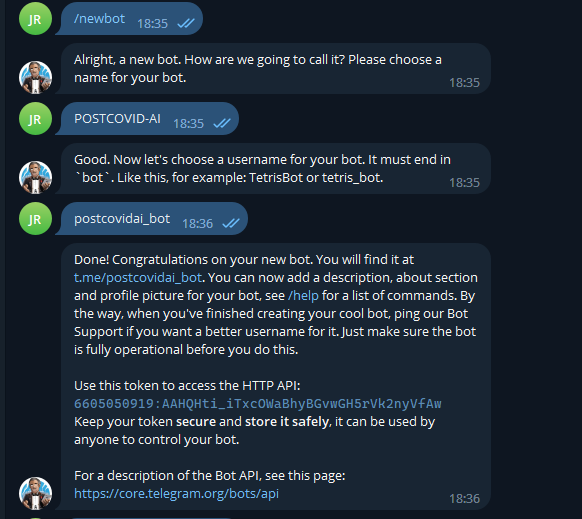
\includegraphics[width=0.7\textwidth, height=8cm]{imagenes/bot_creation.png}
    \caption{ Creación del bot en Telegram }
    \label{fig:planificacion}
\end{figure}


Hecho esto, podemos personalizar nuestro bot como deseemos, cambiando la descripción, el estado, la foto de perfil, comandos personalizados...

\begin{figure}[!ht]
    \centering
    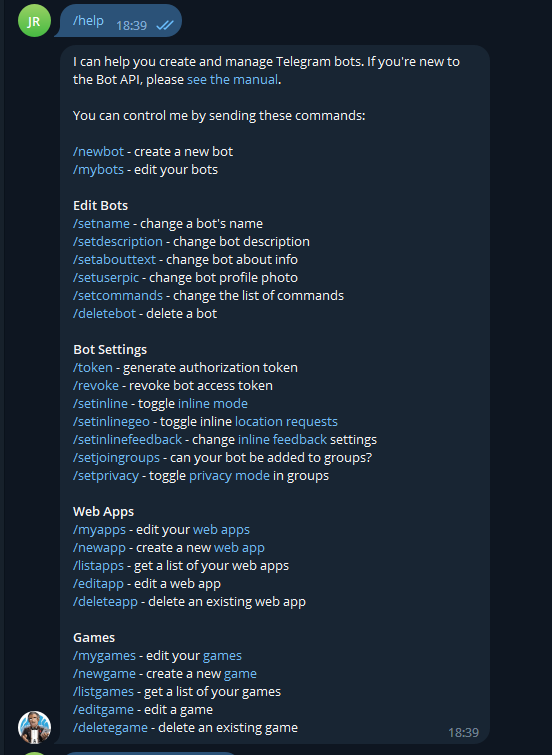
\includegraphics[width=0.8\textwidth, height=9cm]{imagenes/bot_custom.png}
    \caption{ Customización del bot }
    \label{fig:planificacion}
\end{figure}



\section{Instalación}

\subsection{Configuración del entorno}

Antes de explicar como montar el proyecto, son necesarias tener instaladas previamente algunas tecnologías.
La primera de ella es Docker. Dependiendo del sistema operativo que estemos utilizando, debemos descargarlo de una forma u otra. En el caso de Windows, desde la documentación oficial  \textit({\cite{docker})}, nos permite descargar un archivo ejecutable que nos hará la instalación de manera automática. En caso de usar Linux, podemos descargarlo usando los siguientes comandos:

\begin{minted}{bash}
    $ sudo apt-get update
    $ sudo apt-get install ca-certificates curl 
    $ sudo install -m 0755 -d /etc/apt/keyrings
    $ curl -fsSL https://download.docker.com/linux/ubuntu/gpg | sudo gpg 
    --dearmor -o /etc/apt/keyrings/docker.gpg
    $ sudo chmod a+r /etc/apt/keyrings/docker.gpg
    $ echo \
      "deb [arch="$(dpkg --print-architecture)" signed-by=/etc/apt/keyrings/
      docker.gpg] https://download.docker.com/linux/ubuntu \
      "$(. /etc/os-release && echo "$VERSION_CODENAME")" stable" | \
      sudo tee /etc/apt/sources.list.d/docker.list > /dev/null$
    $ sudo apt-get update
    $ sudo apt-get install docker-ce docker-ce-cli containerd.io 
    docker-buildx-plugin docker-compose-plugin
\end{minted}

El lenguaje de programación utilizado es python, por lo que debemos de tenerlo descargado y declarado como variable de entorno en nuestro sistema. En su página oficial, explica como hacerlo \textit({\cite{python})}

El gestor de base de datos utilizado es PostgreSQL. También es posible descargarlo en Windows utilizando del instalador que proveen \textit({\cite{postgres})} o en el caso de Linux ejecutando los siguientes comandos:

\begin{minted}{bash}
    $ sudo sh -c 'echo "deb http://apt.postgresql.org/pub/repos/apt
    $(lsb_release -cs)-pgdg main" > /etc/apt/sources.list.d/pgdg.list'
    $ wget --quiet -O - https://www.postgresql.org/media/keys/ACCC4CF8.asc 
    | sudo apt-key add -
    $ sudo apt-get update
    $ sudo apt-get -y install postgresql
\end{minted}


\subsection{Montaje de desarrollo}

Una vez lo tengamos todo lo necesario, ya podemos pasar al montaje del proyecto. Para ello, descargamos el código del repositorio público de github que contiene el proyecto. Podemos hacerlo a mano o mediante comando.

\begin{minted}{bash}
    $ git clone https://github.com/juantiog22/Thesis.git
\end{minted}

Se ha usado Docker ya que permite entregar código con mayor rapidez, estandarizar las operaciones de las aplicaciones, transferir el código con facilidad y ahorrar dinero al mejorar el uso de recursos. Con Docker, obtiene un solo objeto que se puede ejecutar de manera fiable en cualquier lugar. La sintaxis sencilla y simple de Docker le aporta un control absoluto. Por lo que todo lo necesario a la implantación del proyecto ya se encuentra proporcionado. Dentro de la carpeta de \textit{/Thesis} ejecutamos este comando:

\begin{minted}{bash}
    $ docker-compose up -d --build  
\end{minted}

Esto creará las imágenes de docker correspondientes a la interfaz web, el bot y la base de datos. Además instalará todos los paquetes necesarios situado dentro del archivo \textit{requirements.txt} . 
Para la creación de la base de datos, he exportado la mía que se encuentra dentro del archivo \textit{dumpfile.dump}. Esta base de datos cuenta con preguntas, bloques y contextos previamente creados con ejemplos reales de como serían algunos cuestionarios guiándome según las reglas e información relevante que me proveen desde \textit({\cite{postcovid})}. En el caso de querer establecer esta base de datos tras haber hecho el paso anterior debemos restaurar la nuestra con la información que contiene este archivo. Para ello:

\begin{minted}{bash}
    $ docker-compose exec db bash
    $ pg_restore -U postgres -d postgres dumpfile.dump
\end{minted}

Esto vuelca toda la información en nuestra base de datos y migrará todos los datos de forma automática en la base de datos que provee PostgreSQL por defecto. 

En el caso de no querer usar esa y querer crear otra nueva pero con todos los cambios debemos de crearla previamente. Desde la terminal de psql podemos hacerlo con el siguiente comando:

\begin{minted}{bash}
    $ createdb -U "nombre_propietario" "nombre_base_datos"
\end{minted}

Si hacemos esto, debemos hacer un par de cambios antes de la instalación. En el archivo \textit{docker-compose.yml}, podemos cambiar las variables relacionadas con el entorno de la base de datos antes de construir la imagen.

\begin{minted}{bash}
    - POSTGRES_USER=postgres
    - POSTGRES_DB=postgres
    - POSTGRES_PASSWORD=postgres
\end{minted}

También dentro de la ruta \textit{/telegrambot/telegrambot/settings/local.py} es donde se define la base de datos con la que vamos a trabajar, podemos cambiarlo modificando los parámetros como deseemos. 


\begin{minted}{Python}
DATABASES = {
    'default': {
        'ENGINE': 'django.db.backends.postgresql',
        'NAME': 'postgres',
        'USER': 'postgres',
        'PASSWORD': 'postgres',
        'HOST': 'db',
        'PORT': 5432,
    }
}
\end{minted}

Tendríamos que cambiar los datos relacionados al usuario, contraseña y nombre. 

Si queremos crear una base de datos desde 0 y completamente nueva, simplemente tras construir la imágenes de docker ejecutamos lo siguiente:

\begin{minted}{bash}
    $ docker-compose run web python manage.py makemigrations
    $ docker-compose run web python manage.py migrate
\end{minted}

Esto nos creará una nueva base de datos con todas las tablas correspondiente y lista para funcionar, pero sin ningún registro. 

Una vez todo esté listo, ejecutamos este comando y nuestro proyecto estará corriendo y listo para utilizar.

\begin{minted}{bash}
    $ docker-compose up
\end{minted}

Es importante asegurarse de que no haya otro proceso corriendo en el mismo puerto a la hora de instalarlo para que no nos encontremos con ningún error. Si desde el navegador accedemos a la url: \textit{http://localhost:8000/} podemos acceder a la aplicación web y además el bot se econtrará escuchando y esperando actualizaciones desde la aplicación de Telegram.